% Provenance (never printed): cycle 3 geography and "La planete Terre"
% (the great physical features of the world: relief, rivers, deserts, ice;
% reading a physical map); see sources/book1/PROVENANCE.md.
% Book 1, grade 4, chapter 3.
\chapter{Peta Fisik Dunia}\label{ch:g4:world-physical-map}

Sami dan Noor membentangkan sebuah \omterm{def:g3:continents-and-oceans:world-map}{peta dunia} yang besar di lantai kelas
lalu berlutut mengelilinginya. \omterm{def:g2:drawing-to-map:map}{Peta} ini tidak seperti \omterm{def:g2:drawing-to-map:map}{peta} yang mereka
kenal. Tidak ada negara, tidak ada perbatasan, dan tidak ada kota.
Sebaliknya, daratannya diwarnai: hijau di sepanjang \omterm{def:g1:landscapes-around-us:water}{pesisir} dan di
\omterm{def:g1:landscapes-around-us:landform}{dataran-dataran} luas, lalu kuning pucat, lalu cokelat, dan di beberapa
tempat hampir putih. \omterm{def:g2:water-on-earth:ocean}{Lautnya} pun punya beberapa warna biru: pucat di dekat
\omterm{def:g1:landscapes-around-us:water}{pesisir}, lalu makin lama makin tua jauh di tengah \omterm{def:g2:water-on-earth:ocean}{samudra}.

``Kenapa bagian Asia itu putih?'' tanya Noor. ``Apakah itu \omterm{def:g4:clouds-rain-snow:precipitation}{salju}?'' Bukan
begitu. Di \omterm{def:g2:drawing-to-map:map}{peta} ini, setiap warna menunjukkan seberapa tinggi daratan, atau
seberapa dalam \omterm{def:g2:water-on-earth:ocean}{laut}.

\begin{recall}
\omterm{def:g2:drawing-to-map:map}{Peta} menggambarkan suatu tempat dilihat dari atas, dibuat lebih kecil;
\omterm{def:g2:drawing-to-map:legend}{legendanya} menjelaskan warna dan simbolnya (\cref{ch:g2:drawing-to-map}).
Daratan terkumpul dalam tujuh \omterm{def:g3:continents-and-oceans:continent}{benua}, di antara lima \omterm{def:g2:water-on-earth:ocean}{samudra}, dan \omterm{def:g3:continents-and-oceans:world-map}{peta dunia}
adalah \omterm{def:g3:continents-and-oceans:globe}{bola dunia} yang dibentangkan menjadi datar
(\cref{ch:g3:continents-and-oceans}). \omterm{def:g1:landscapes-around-us:landform}{Gunung}, \omterm{def:g1:landscapes-around-us:landform}{bukit}, \omterm{def:g1:landscapes-around-us:landform}{lembah}, dan \omterm{def:g1:landscapes-around-us:landform}{dataran}
adalah \omterm{def:g1:landscapes-around-us:landform}{bentuk muka bumi}; \omterm{def:g1:landscapes-around-us:water}{sungai} mengalir dari daratan tinggi turun ke \omterm{def:g2:water-on-earth:ocean}{laut}
(\cref{ch:g1:landscapes-around-us}).
\end{recall}

\section{Membaca peta fisik}

Untuk menyatakan seberapa tinggi suatu tempat, kita memerlukan \omterm{def:g4:world-physical-map:altitude}{ketinggian}
awal yang sama di mana pun di Bumi. Kita memakai \omterm{def:g4:world-physical-map:altitude}{ketinggian} \omterm{def:g4:world-physical-map:altitude}{permukaan laut}.

\begin{definition}[Ketinggian dan permukaan laut]\label{def:g4:world-physical-map:altitude}
Yang disebut \emph{permukaan laut}\index{permukaan laut} adalah ketinggian
rata-rata permukaan \omterm{def:g2:water-on-earth:ocean}{laut}, di antara pasang naik dan pasang surut. Yang
disebut \emph{ketinggian}\index{ketinggian} suatu tempat adalah tingginya di
atas permukaan \omterm{def:g2:water-on-earth:ocean}{laut}, dalam meter. Di bawah \omterm{def:g2:water-on-earth:ocean}{laut}, kita berbicara tentang
\emph{kedalaman}: seberapa jauh dasar \omterm{def:g2:water-on-earth:ocean}{laut} terletak di bawah permukaan \omterm{def:g2:water-on-earth:ocean}{laut}.
\end{definition}

Kota di tepi \omterm{def:g2:water-on-earth:ocean}{laut} mempunyai \omterm{def:g4:world-physical-map:altitude}{ketinggian} beberapa meter. Desa di \omterm{def:g4:world-physical-map:range}{pegunungan}
bisa terletak pada 1\,500 meter: satu setengah kilometer di atas \omterm{def:g4:world-physical-map:altitude}{permukaan
laut}, walaupun desa itu berjarak ratusan kilometer dari \omterm{def:g1:landscapes-around-us:water}{pesisir} mana pun.

\begin{definition}[Relief]\label{def:g4:world-physical-map:relief}
Yang disebut \emph{relief}\index{relief} suatu wilayah adalah bentuk
daratannya: bagian yang tinggi dan bagian yang rendah, \omterm{def:g1:landscapes-around-us:landform}{gunung-gunungnya},
dataran tingginya, \omterm{def:g1:landscapes-around-us:landform}{lembah-lembahnya}, dan dataran rendahnya.
\end{definition}

\begin{definition}[Peta fisik]\label{def:g4:world-physical-map:physical-map}
Yang disebut \emph{peta fisik}\index{peta fisik} menunjukkan \omterm{def:g4:world-physical-map:relief}{relief} daratan
dan kedalaman \omterm{def:g2:water-on-earth:ocean}{laut} dengan warna, satu warna untuk setiap jenjang \omterm{def:g4:world-physical-map:altitude}{ketinggian}
atau kedalaman, beserta \omterm{def:g1:landscapes-around-us:water}{sungai-sungai} besar, \omterm{def:g1:landscapes-around-us:water}{danau}, gurun, dan es.
\end{definition}

\begin{omfigure}
\begin{tikzpicture}
\begin{axis}[ommap, width=\linewidth, xtick=\empty, ytick=\empty, grid=none,
    axis background/.style={}, clip=true]
  \addplot graphics[xmin=-180, xmax=180, ymin=-90, ymax=90]
    {figdata/out/grade-4-physical_map.png};
  \addplot[black!45, line width=0.15pt] table {figdata/out/shared-geo-land.dat};
  \addplot[fill=omHypsSeaB, draw=blue!60!black, line width=0.2pt]
    table {figdata/out/grade-4-physical_map-lakes.dat};
  \addplot[blue!70!black, line width=0.5pt] table {figdata/out/grade-4-physical_map-rivers.dat};
  \begin{scope}[every node/.style={font=\scriptsize\bfseries, align=center,
      fill=white, fill opacity=0.7, text opacity=1, inner sep=1pt, rounded corners=1pt}]
    \node at (axis cs:-112,47) {Pegunungan\\Rocky};
    \node at (axis cs:-62,-22) {Andes};
    \node at (axis cs:10,49) {Alpen};
    \node at (axis cs:84,24) {Himalaya};
    \node at (axis cs:4,23) {Sahara};
    \node at (axis cs:-40,74) {Greenland\\(es)};
    \node at (axis cs:60,-80) {Antarktika (es)};
  \end{scope}
  \begin{scope}[every node/.style={font=\scriptsize\itshape, text=blue!50!black,
      fill=white, fill opacity=0.6, text opacity=1, inner sep=1pt}]
    \node at (axis cs:38,17) {Nil};
    \node at (axis cs:-56,-7) {Amazon};
    \node at (axis cs:-80,33) {Mississippi};
    \node at (axis cs:118,26) {Yangtze};
  \end{scope}
\end{axis}
\end{tikzpicture}

\smallskip
\begin{tikzpicture}[font=\scriptsize, x=1.18cm]
  \foreach \i/\c/\t in {0/5A9CCF/{lebih dari\\4000}, 1/84BCE0/{2000\\s.d. 4000},
      2/B3D8EE/{200\\s.d. 2000}, 3/DCEEF8/{0\\s.d. 200}} {
    \definecolor{tmp}{HTML}{\c}
    \fill[tmp, draw=black!40] (\i,0) rectangle (\i+0.92,0.35);
    \node[align=center, anchor=north] at (\i+0.45,-0.05) {\t};
  }
  \foreach \i/\c/\t in {5/9CC98A/{0\\s.d. 200}, 6/C9DE99/{200\\s.d. 500},
      7/F1E7A8/{500\\s.d. 1000}, 8/E5C58A/{1000\\s.d. 2000}, 9/C79E76/{2000\\s.d. 4000},
      10/ECE8E3/{lebih dari\\4000}} {
    \definecolor{tmp}{HTML}{\c}
    \fill[tmp, draw=black!40] (\i,0) rectangle (\i+0.92,0.35);
    \node[align=center, anchor=north] at (\i+0.45,-0.05) {\t};
  }
  \node[anchor=south] at (2,0.4) {kedalaman laut (m)};
  \node[anchor=south] at (8,0.4) {ketinggian daratan (m)};
\end{tikzpicture}

{\small \omterm{def:g4:world-physical-map:physical-map}{Peta fisik} dunia, beserta \omterm{def:g2:drawing-to-map:legend}{legendanya}. Setiap warna adalah satu
jenjang \omterm{def:g4:world-physical-map:altitude}{ketinggian} (di darat) atau kedalaman (di bawah \omterm{def:g2:water-on-earth:ocean}{laut}). \omterm{def:g1:landscapes-around-us:water}{Sungai}
digambar dengan biru tua. \omterm{def:g4:world-physical-map:relief}{Relief} digambar dari satu nilai untuk setiap
derajat lintang dan bujur (kira-kira setiap 100 kilometer), sehingga
tampak dihaluskan: puncak tunggal dan palung yang sempit tidak terlihat.
Data: \omterm{def:g4:world-physical-map:relief}{relief} NOAA ETOPO1; \omterm{def:g1:landscapes-around-us:water}{sungai}, \omterm{def:g1:landscapes-around-us:water}{danau}, dan garis pantai dari Natural
Earth.}
\label{fig:g4:world-physical-map:map}
% ledger: data:etopo1, data:b1-ne-rivers, data:ne-land
\end{omfigure}

\begin{method}[Membaca warna pada peta fisik]\label{met:g4:world-physical-map:reading}
Untuk mencari \omterm{def:g4:world-physical-map:altitude}{ketinggian} suatu tempat pada \omterm{def:g4:world-physical-map:physical-map}{peta fisik}:
\begin{enumerate}
  \item cari tempat itu, lalu perhatikan warnanya;
  \item cari warna yang sama di \omterm{def:g2:drawing-to-map:legend}{legenda};
  \item baca jenjang di bawahnya: \omterm{def:g4:world-physical-map:altitude}{ketinggian} tempat itu terletak di antara
        kedua angka tersebut.
\end{enumerate}
Cara yang sama berlaku di \omterm{def:g2:water-on-earth:ocean}{laut}, untuk kedalaman.
\end{method}

\begin{example}[Tiga tempat]\label{ex:g4:world-physical-map:three}
Muara \omterm{def:g1:landscapes-around-us:water}{Sungai} Amazon, di \omterm{def:g1:landscapes-around-us:water}{pesisir} Amerika Selatan, berwarna hijau tua:
\omterm{def:g4:world-physical-map:altitude}{ketinggiannya} antara 0 dan 200 meter. Bagian tengah Sahara berwarna hijau
pucat atau kuning pucat: antara 200 dan 1\,000 meter. Dataran tinggi di
utara Himalaya, di Asia, hampir putih: lebih dari 4\,000 meter.
\end{example}

\section{Pegunungan-pegunungan besar}

Di \omterm{def:g2:drawing-to-map:map}{peta}, warna cokelat dan putih tidak tersebar merata. Warna-warna itu
membentuk jalur-jalur yang panjang dan sempit.

\begin{definition}[Pegunungan]\label{def:g4:world-physical-map:range}
Yang disebut \emph{pegunungan}\index{pegunungan} adalah deretan panjang
\omterm{def:g1:landscapes-around-us:landform}{gunung} yang bersambung satu sama lain, yang membentang sejauh ratusan atau
ribuan kilometer.
\end{definition}

\omterm{def:g4:world-physical-map:range}{Pegunungan} Andes membentang di sepanjang sisi barat Amerika Selatan. Di
Amerika Utara ada \omterm{def:g4:world-physical-map:range}{Pegunungan} Rocky, di Eropa ada \omterm{def:g4:world-physical-map:range}{Pegunungan} Alpen, dan di
Asia ada yang tertinggi di antara semuanya: Himalaya. Di sanalah
berdiri \omterm{def:g1:landscapes-around-us:landform}{gunung} tertinggi di Bumi: Gunung Everest, setinggi 8\,849 meter,
yang diukur ulang pada tahun 2020.
% ledger: tht:everest

\begin{omfigure}
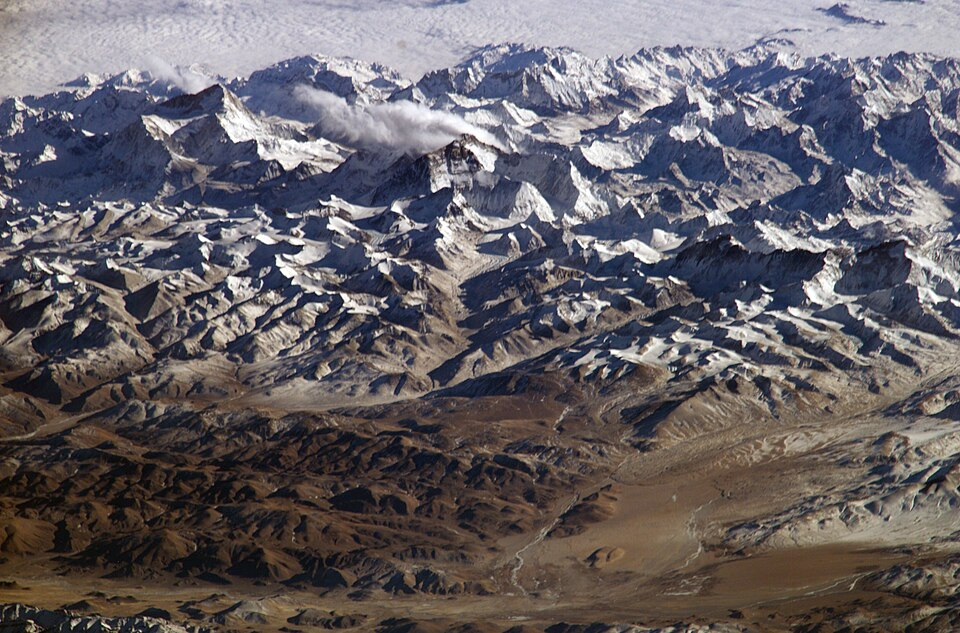
\includegraphics[width=0.75\linewidth]{images/book1/g4-himalaya-iss.jpg}

{\small Himalaya dilihat dari Stasiun Antariksa Internasional, menghadap ke
selatan dari dataran tinggi Tibet: lautan puncak yang tertutup \omterm{def:g4:clouds-rain-snow:precipitation}{salju}.
Foto: NASA (domain publik).}
% ledger: nasa:himalaya-iss
\end{omfigure}

\section{Sungai dan danau besar}

Air \omterm{def:g4:clouds-rain-snow:precipitation}{hujan} dan \omterm{def:g4:clouds-rain-snow:precipitation}{salju} yang mencair mengalir di permukaan tanah, berkumpul
menjadi \omterm{def:g1:landscapes-around-us:water}{sungai-sungai} kecil lalu menjadi \omterm{def:g1:landscapes-around-us:water}{sungai}, dan \omterm{def:g1:landscapes-around-us:water}{sungai} membawa air itu
turun ke \omterm{def:g2:water-on-earth:ocean}{laut}. \omterm{def:g1:landscapes-around-us:water}{Sungai-sungai} terbesar menampung air dari seluruh wilayah
suatu \omterm{def:g3:continents-and-oceans:continent}{benua}.

Dua \omterm{def:g1:landscapes-around-us:water}{sungai} terpanjang di Bumi adalah \omterm{def:g1:landscapes-around-us:water}{Sungai} Nil, di Afrika, dan \omterm{def:g1:landscapes-around-us:water}{Sungai}
Amazon, di Amerika Selatan. Panjang masing-masing hampir 7\,000 kilometer.
Mana yang paling panjang? Tidak ada yang tahu dengan pasti, karena hal itu
bergantung pada tempat yang kita anggap sebagai awal sebuah \omterm{def:g1:landscapes-around-us:water}{sungai}: di antara
semua \omterm{def:g1:landscapes-around-us:water}{sungai} kecil yang bergabung membentuknya, mana yang dihitung
sebagai awalnya yang sebenarnya? Pada tahun 2007, sebuah tim yang menelusuri
Amazon sampai ke sumber yang lebih jauh menyatakan bahwa panjangnya
kira-kira 6\,800 kilometer, sedikit lebih panjang daripada Nil; banyak buku
rujukan masih menyebut Nil sebagai yang terpanjang.
% ledger: natgeo:nile, natgeo:amazon-nile-2007

Amazon, tanpa keraguan sedikit pun, adalah \omterm{def:g1:landscapes-around-us:water}{sungai} terbesar: \omterm{def:g1:landscapes-around-us:water}{sungai} ini
membawa air lebih banyak daripada \omterm{def:g1:landscapes-around-us:water}{sungai} mana pun.
% ledger: natgeo:amazon-nile-2007

\begin{omfigure}
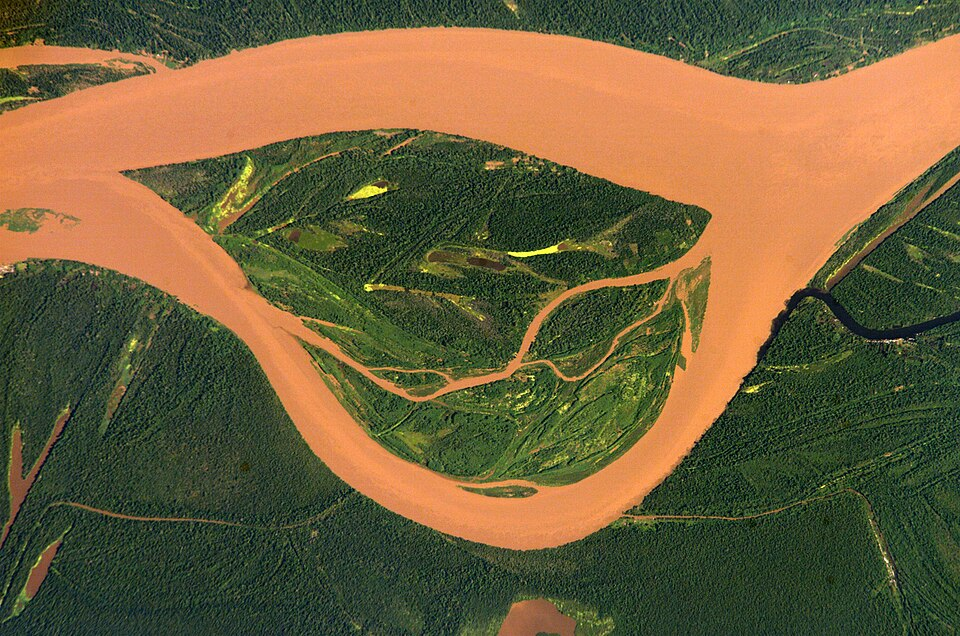
\includegraphics[width=0.6\linewidth]{images/book1/g4-amazon-iss.jpg}

{\small \omterm{def:g1:landscapes-around-us:water}{Sungai} Amazon, cokelat oleh \omterm{def:g3:stones-pebbles-sand:sand}{lumpur}, berkelok-kelok di tengah hutan
\omterm{def:g4:clouds-rain-snow:precipitation}{hujan}, dilihat dari Stasiun Antariksa Internasional. Foto: NASA (domain
publik).}
% ledger: nasa:amazon-iss
\end{omfigure}

\omterm{def:g1:landscapes-around-us:water}{Danau} pun memecahkan rekor. \omterm{def:g1:landscapes-around-us:water}{Danau} terbesar di Bumi adalah \omterm{def:g2:water-on-earth:ocean}{Laut} Kaspia, di
antara Eropa dan Asia: \omterm{def:g1:landscapes-around-us:water}{danau} ini begitu besar sehingga disebut \omterm{def:g2:water-on-earth:ocean}{laut}, tetapi
ia dikelilingi daratan di semua sisinya. Luasnya lebih dari
370\,000 kilometer persegi. \omterm{def:g1:landscapes-around-us:water}{Danau} terdalam adalah \omterm{def:g1:landscapes-around-us:water}{Danau} Baikal, di Rusia: di
beberapa tempat dasarnya terletak hampir 2 kilometer di bawah permukaannya.
% ledger: natgeo:caspian-baikal

\section{Gurun dan es raksasa}

Dua jenis tempat tampak menonjol pada \omterm{def:g4:world-physical-map:physical-map}{peta fisik} karena hampir tidak ada yang
tumbuh di sana: gurun-gurun besar, tempat \omterm{def:g4:clouds-rain-snow:precipitation}{hujan} hampir tidak pernah turun, dan
es raksasa.

Sahara, di utara Afrika, adalah gurun panas terbesar di Bumi. Luasnya
kira-kira delapan setengah juta kilometer persegi. Seluruh Afrika luasnya
kira-kira 30 juta kilometer persegi, jadi Sahara sedikit lebih dari
seperempat \omterm{def:g3:continents-and-oceans:continent}{benua} itu: lebih dari $\frac{1}{4}$, tetapi kurang dari
$\frac{1}{3}$.
% ledger: natgeo:sahara, data:etopo1

Es raksasa menutupi Antarktika, di sekitar \omterm{def:g3:continents-and-oceans:poles}{Kutub Selatan}, dan sebagian besar
Greenland, di ujung utara \omterm{def:g2:water-on-earth:ocean}{Samudra} Atlantik. Di sana, \omterm{def:g4:clouds-rain-snow:precipitation}{salju} dari ribuan tahun
telah menumpuk dan berubah menjadi lapisan es yang tebal. Pada \omterm{def:g4:world-physical-map:physical-map}{peta fisik},
warnanya adalah warna daratan tinggi, karena permukaan esnya terletak jauh
di atas \omterm{def:g4:world-physical-map:altitude}{permukaan laut}.

\section{Yang tertinggi dan yang terdalam}

\omterm{def:g4:world-physical-map:physical-map}{Peta fisik} menunjukkan bentuk permukaan Bumi, tetapi \omterm{def:g2:drawing-to-map:map}{peta} itu begitu kecil
sehingga menyembunyikan titik-titik ekstremnya. Mari kita letakkan
titik-titik itu berdampingan, dengan skala yang sama.

\begin{omfigure}
\begin{tikzpicture}[x=1cm, y=0.32cm, font=\small]
  % sea level
  \fill[omHypsSeaA] (0,0) rectangle (9,-11.5);
  \fill[omHypsSeaD!80] (4.6,-11.5) -- (4.6,-11.0) -- (5.0,-10.98) -- (5.4,-11.0) -- (5.4,-11.5) -- cycle;
  \draw[black!60] (-0.2,0) -- (9.2,0);
  \node[anchor=west, font=\scriptsize] at (9.25,0) {permukaan laut, 0\,m};
  % height scale
  \draw[black!60] (0,-11.5) -- (0,10);
  \foreach \h in {-10,-8,...,8} {
    \draw[black!60] (-0.1,\h) -- (0,\h);
    \node[anchor=east, font=\scriptsize] at (-0.12,\h) {\h\,km};
  }
  % ocean floor and trench
  \fill[brown!45] (0.05,-11.5) -- (0.05,-3.7) -- (3.2,-3.7) -- (4.4,-6) -- (4.9,-10.98) -- (5.1,-10.98)
    -- (5.6,-6) -- (6.4,-3.7) -- (9,-3.7) -- (9,-11.5) -- cycle;
  \node[font=\scriptsize, align=center] at (2.0,-5.3) {dasar samudra,\\kedalaman sekitar 3\,700\,m};
  \node[font=\scriptsize, anchor=west, align=left] at (5.6,-9.4) {titik terdalam:\\Challenger Deep,\\hampir 11\,000\,m};
  % Everest
  \fill[black!35] (6.6,0) -- (7.6,8.85) -- (8.6,0) -- cycle;
  \fill[white, draw=black!45, line width=0.3pt] (7.35,6.6) -- (7.6,8.85) -- (7.85,6.6) -- (7.6,7.1) -- cycle;
  \node[font=\scriptsize, align=center, anchor=south] at (7.6,8.95) {Gunung Everest, 8\,849\,m};
  % cirrus clouds band
  \draw[black!45, line width=0.6pt] (1.0,9.0) .. controls (1.6,9.5) and (2.2,9.1) .. (2.8,9.6);
  \draw[black!45, line width=0.6pt] (1.2,8.3) .. controls (1.8,8.8) and (2.4,8.4) .. (3.0,8.9);
  \node[font=\scriptsize, align=center] at (2.0,7.2) {awan tinggi\\(sirus)};
  % a village
  \fill[black!60] (2.2,1.5) rectangle (2.45,1.75);
  \node[font=\scriptsize, anchor=west] at (2.5,1.6) {desa pegunungan, 1\,500\,m};
\end{tikzpicture}

{\small Dari titik terdalam \omterm{def:g2:water-on-earth:ocean}{samudra} sampai puncak tertinggi, dengan skala
yang sebenarnya. Challenger Deep, di \omterm{def:g2:water-on-earth:ocean}{Samudra} Pasifik, terletak lebih dalam
di bawah \omterm{def:g2:water-on-earth:ocean}{laut} daripada tinggi Gunung Everest di atasnya. Nilai: Everest
8\,849\,m; Challenger Deep hampir 11\,000\,m; dasar \omterm{def:g2:water-on-earth:ocean}{samudra} rata-rata
kira-kira 3\,700\,m.}
\label{fig:g4:world-physical-map:extremes}
% ledger: tht:everest, usgs:trench-depth, nos:ocean-depth, wmo:cloud-levels
\end{omfigure}

\begin{example}[Everest di kedalaman]\label{ex:g4:world-physical-map:everest-in-deep}
Seandainya kita bisa mengangkat Gunung Everest dan meletakkannya di dasar
Challenger Deep, puncaknya masih akan berada di bawah air: kira-kira
11\,000 meter palung, dibandingkan dengan 8\,849 meter \omterm{def:g1:landscapes-around-us:landform}{gunung}. Lebih dari 2
kilometer air \omterm{def:g2:water-on-earth:ocean}{laut} masih akan menutupinya.
% ledger: tht:everest, usgs:trench-depth
\end{example}

\section{Latihan}

\begin{exercise}[$\star$]\label{exo:g4:world-physical-map:1}
Apa yang dimaksud dengan \omterm{def:g4:world-physical-map:altitude}{ketinggian} suatu tempat? Dari \omterm{def:g4:world-physical-map:altitude}{ketinggian} manakah \omterm{def:g4:world-physical-map:altitude}{ketinggian} itu diukur?
\end{exercise}

\begin{exercise}[$\star$]\label{exo:g4:world-physical-map:2}
Dengan memakai \omterm{def:g2:drawing-to-map:legend}{legenda} \omterm{def:g4:world-physical-map:physical-map}{peta fisik}, sebutkan \omterm{def:g4:world-physical-map:altitude}{ketinggian} tempat yang
berwarna: (a) hijau tua; (b) kuning pucat; (c) hampir putih.
\end{exercise}

\begin{exercise}[$\star$]\label{exo:g4:world-physical-map:3}
Di \omterm{def:g3:continents-and-oceans:continent}{benua} manakah letak: (a) \omterm{def:g4:world-physical-map:range}{Pegunungan} Andes; (b) Himalaya; (c) Sahara;
(d) \omterm{def:g4:world-physical-map:range}{Pegunungan} Rocky?
\end{exercise}

\begin{exercise}[$\star$]\label{exo:g4:world-physical-map:4}
Sebutkan \omterm{def:g1:landscapes-around-us:landform}{gunung} tertinggi di Bumi, \omterm{def:g1:landscapes-around-us:water}{danau} terbesar, dan \omterm{def:g1:landscapes-around-us:water}{danau} terdalam.
\end{exercise}

\begin{exercise}[$\star$]\label{exo:g4:world-physical-map:5}
Pada \omterm{def:g4:world-physical-map:physical-map}{peta fisik}, \omterm{def:g2:water-on-earth:ocean}{laut} di dekat \omterm{def:g1:landscapes-around-us:water}{pesisir} berwarna biru pucat dan bagian
tengah \omterm{def:g2:water-on-earth:ocean}{samudra} berwarna biru tua. Apa yang dapat kamu simpulkan tentang
kedalaman \omterm{def:g2:water-on-earth:ocean}{laut}?
\end{exercise}

\begin{exercise}[$\star$]\label{exo:g4:world-physical-map:6}
Mengapa Antarktika dan Greenland diwarnai seperti daratan tinggi pada \omterm{def:g4:world-physical-map:physical-map}{peta
fisik}?
\end{exercise}

\begin{exercise}[$\star\star$]\label{exo:g4:world-physical-map:7}
Urutkan, dari yang terendah sampai yang tertinggi: sebuah pantai; sebuah
desa pada 1\,500 meter; puncak Gunung Everest; dasar Challenger Deep; dasar
\omterm{def:g2:water-on-earth:ocean}{samudra} rata-rata.
\end{exercise}

\begin{exercise}[$\star\star$]\label{exo:g4:world-physical-map:8}
Mengapa kita tidak bisa memastikan apakah Nil atau Amazon yang merupakan
\omterm{def:g1:landscapes-around-us:water}{sungai} terpanjang?
\end{exercise}

\begin{exercise}[$\star\star$]\label{exo:g4:world-physical-map:9}
Afrika luasnya kira-kira 30 juta kilometer persegi. Berapa seperempatnya?
Berapa sepertiganya? Sahara luasnya kira-kira delapan setengah juta
kilometer persegi: apakah lebih atau kurang dari seperempat Afrika? Lebih
atau kurang dari sepertiganya?
\end{exercise}

\begin{exercise}[$\star\star$]\label{exo:g4:world-physical-map:10}
Sebuah pondok \omterm{def:g1:landscapes-around-us:landform}{gunung} terletak pada 2\,500 meter, dan sebuah \omterm{def:g1:landscapes-around-us:water}{danau} di
bawahnya pada 1\,000 meter. Berapa meter lebih tinggi pondok itu? Warna
apa yang dimiliki keduanya pada \omterm{def:g4:world-physical-map:physical-map}{peta fisik}?
\end{exercise}

\begin{exercise}[$\star\star\star$]\label{exo:g4:world-physical-map:11}
Sebuah pesawat terbang 10 kilometer di atas \omterm{def:g4:world-physical-map:altitude}{permukaan laut}. Apakah pesawat
itu lebih tinggi daripada Gunung Everest? Lebih tinggi berapa meter? Jika
pesawat itu terbang di atas Challenger Deep, berapa jauh jaraknya dari dasar
palung (anggap palung itu 11\,000 meter)?
\end{exercise}
